\documentclass{beamer}

% You can also use a 16:9 aspect ratio:
%\documentclass[aspectratio=169]{beamer}
\usetheme{TACC16}
\usepackage{graphicx}

% It's possible to move the footer to the right:
%\usetheme[rightfooter]{TACC16}


% Detailed knowledge of application workload characteristics can
% optimize performance of current and future systems. This may sound
% daunting, with many HPC data centers hosting over 2,000 users running
% thousands of applications and millions of jobs per month.  XALT is an
% open source tool developed at the Texas Advanced Computing Center
% (TACC) that collects system usage information to quantitatively report
% how users are using your system. This session will explore the
% benefits of detailed application workload profiling and how the XALT
% tool has helped leading supercomputing sites unlock the power of their
% application usage data.

%% page 
%\begin{frame}{}
%  \begin{itemize}
%    \item
%  \end{itemize}
%\end{frame}
%
%% page 
%\begin{frame}[fragile]
%    \frametitle{}
% {\tiny
%    \begin{semiverbatim}
%    \end{semiverbatim}
%}
%  \begin{itemize}
%    \item
%  \end{itemize}
%
%\end{frame}



\begin{document}
\title[XALT]{10 years of XALT: A Retrospective}
\author{Robert McLay}
\date{August 17, 2023}

% page 1
\frame{\titlepage}

% page 2
\begin{frame}{XALT: Outline}
  \center{
\includegraphics[width=.9\textwidth]{XALT_Sticker.png}}
  \begin{itemize}
    \item History: Lariat and ALTD
    \item XALT 1 funded by NSF
    \item XALT 2
    \item Sharing Memory and Namespace with every program run on the
      system
    \item Lessons learn from running an Open Source Project
    \item Conclusions
  \end{itemize}
\end{frame}

%page 3
\begin{frame}{History}
  \begin{itemize}
    \item My Boss, John Cazes, asked if I could track what MPI
      executable ran on our system
    \item I added code around our ibrun submission tool (AKA our mpirun/srun)
    \item Could do some tracking but no database
    \item Lariat was born (was LASSO but name conflict)
  \end{itemize}
\end{frame}

% page 4
\begin{frame}{XALT History}
  \begin{itemize}
    \item Mark Fahey contacted us at TACC for a joint proposal
    \item With an amazing amount of help from my colleague Doug James
    \item Mark and I joined forces to submit a successful NSF proposal
      in 2013.
    \item XALT combined the best parts of both projects (ALTD and
      Lariat)
    \item The name XALT comes from eXtended ALTd (suggested by Doug
      James)
    \item Originally UTWrangler but name conflict again.
  \end{itemize}
\end{frame}

% page 5
\begin{frame}{XALT I}
  \begin{itemize}
    \item It only tracked MPI executions
    \item It did have a database
    \item It tracked Linking of executable
    \item Used UUID (universal unique id) to connect links to execution
    \item Rather than making calls to database like ALTD did
    \item It mainly used Python to collect data (a bad idea)
  \end{itemize}
\end{frame}


% page 6
\begin{frame}{XALT 2}
  \begin{itemize}
    \item My friend and colleague, Bill Barth, found this ELF trick.
    \item One could modify the execution of non-static execution.
    \item By using LD\_PRELOAD and a shared library.
    \item There are similar ways under macOS but ...
  \end{itemize}
\end{frame}

% page 7
\begin{frame}[fragile]
    \frametitle{How XALT 2 works}
 {\tiny
    \begin{semiverbatim}
#include <stdio.h>
void myinit(int argc, char **argv)
\{ printf("This is run before main()\textbackslash{}n"); \}
void myfini()
\{ printf("This is run after main()\textbackslash{}n"); \}

__attribute__((section(".init_array"))) __typeof__(myinit) *__init = myinit;
__attribute__((section(".fini_array"))) __typeof__(myfini) *__fini = myfini;
    \end{semiverbatim}
}
  \begin{itemize}
    \item my\_docs/22/xalt\_monthly\_mtg\_2022\_03\_17/code/bad\_memory/ex1
  \end{itemize}
\end{frame}

% page 8
\begin{frame}[fragile]
    \frametitle{How XALT works (II)}
 {\small
    \begin{semiverbatim}
\% cat try.c

#include <stdio.h>
int main()
\{
  printf("Hello World!\textbackslash{}n");
  return 0;
\}

    \end{semiverbatim}
}
\end{frame}


% page 9
\begin{frame}[fragile]
    \frametitle{How XALT works (III)}
 {\small
    \begin{semiverbatim}
\$ ./try

Hello World!

\$ LD\_PRELOAD=./libxalt.so  ./try
This is run before main()
Hello World!
This is run after main()
    \end{semiverbatim}
}
  \begin{itemize}
    \item my\_docs/22/xalt\_monthly\_mtg\_2022\_03\_17/code/bad\_memory/ex1
  \end{itemize}

\end{frame}

% page 10
\begin{frame}{Hijacking the linker}
  \begin{itemize}
    \item XALT uses Lmod to put its ld early in the path
    \item This doesn't work with llvm compilers
    \item Sites have to move llvm's ld to ld.x and place XALT's ld in
      the right place
  \end{itemize}
\end{frame}

% page 11
\begin{frame}{Implications of tracking everything}
  \begin{itemize}
    \item Too much data!! $\Rightarrow$ Sampling
    \item Being in the same namespace of your program
    \item Sharing memory allocation with your program.
    \item Feeling like I'm a developer on every program team.
  \end{itemize}
\end{frame}

% page 12
\begin{frame}{Sharing Namespace}
  \begin{itemize}
    \item XALT uses xalt\_obfuscate.h to hide the xalt library
      (libxalt\_init.so)
    \item This sharing is common with all libraries
    \item But usually it is opt-in.
    \item But very few libraries are uses everywhere, except libc.so
  \end{itemize}
\end{frame}

% page 13
\begin{frame}[fragile]
    \frametitle{Hiding XALT routine names from users}
 {\tiny
    \begin{semiverbatim}
\% nm \$LD\_PRELOAD| grep \_\_XALT\_build
0000000000009e80 T \_\_XALT\_buildEnvT\_xalt\_1\_5
000000000000a840 T \_\_XALT\_buildUserT\_xalt\_1\_5
00000000000163a0 T \_\_XALT\_buildXALTRecordT\_xalt\_1\_5
    \end{semiverbatim}
}
  \begin{itemize}
    \item XALT routine names are hidden by macros supplied in xalt\_obfuscate.h
  \end{itemize}

\end{frame}


% page 14
\begin{frame}{Cannot hide routines in system libraries like libuuid}
  \begin{itemize}
    \item The routine ``\textbf{random}'' is used by libuuid.so
    \item A user's program created their own random routine in fortran
    \item The program crash when XALT was used.
    \item Solution: use dynamic linking via libdl.so for libuuid.so
      and others.
  \end{itemize}
\end{frame}


% page 15
\begin{frame}{User's bug hidden by initially zeroed memory}
  \begin{itemize}
    \item Initially all memory is zeroed before program starts
    \item Note that pointer zero, integer zero and float zero are all
      zero bits
    \item Link lists require a NULL pointer at end of list.
    \item Used memory is {\color{red} \emph{NOT}} zeroed for you in C.
    \item User's program work w/o XALT, Failed with XALT.
    \item XALT Fix was to zero memory before returning it
    \item Also only return memory when necessary
  \end{itemize}
\end{frame}

% page 16
\begin{frame}{XALT has been a group effort}
  \begin{itemize}
    \item James McComb \& Michael Scott from IU $\Rightarrow$ Tracking R imports
    \item Kenneth Hoste $\Rightarrow$ Riccardo Murri $\Rightarrow$
      Tracking Python imports
    \item Bill Barth $\Rightarrow$ Tracking MATLAB imports
    \item NVIDIA's Scott McMillan $\Rightarrow$ Tracking NVIDIA GPU
      usage
    \item Bilel Hadri $\Rightarrow$ ALTD at NICS
    \item Doug James wrote the NSF proposal with help from Mark and me
    \item See ACKNOWLEDGMENTS.txt for a complete list
  \end{itemize}
\end{frame}

% page 17
\begin{frame}{Lessons Learned}
  \begin{itemize}
    \item Figuring out how to debug on a remote site via XALT\_TRACING=  
    \item Reporting the XALT configuration
    \item make gittag TAG=...; make world\_update
    \item git worktrees
    \item Exploiting Lmod to help XALT (reverse map: path
      $\Rightarrow$ to module)
    \item Using python config files to build C code.
    \item Speed, Speed, Speed
    \item Building trust with the user community
  \end{itemize}
\end{frame}

% page 18
\begin{frame}{Building trust with the user community}
  \begin{itemize}
    \item Making it reliable via Testing
    \item Timely answering the email and github issues 
    \item Book: Team Geek
    \item Learning to be polite when answering and re-answering
      questions
    \item ``You might consider ...''
    \item ``Please test XALT version ... when you get a chance to see
      if it works for you''
    \item Not getting upset when non-native English speakers sound
      insulting
  \end{itemize}
\end{frame}

% page 19
\begin{frame}[fragile]
    \frametitle{XALT Doc usage by City}
    \center{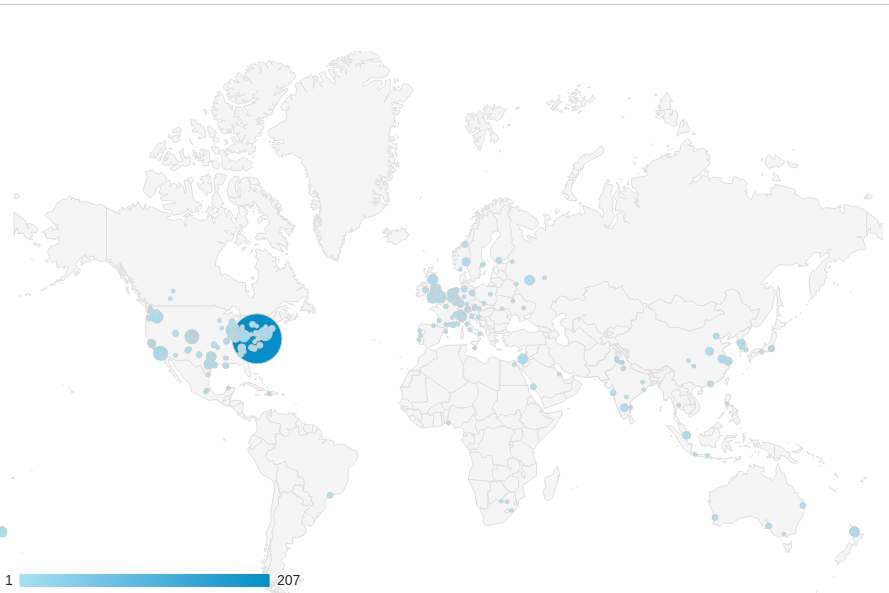
\includegraphics[width=.9\textwidth]{XALT_doc_usage_by_city}}
\end{frame}

% page 20
\begin{frame}{Conclusions}
  \begin{itemize}
    \item It has been quite the learning experience
    \item XALT is considerable better for being Open Source
  \end{itemize}
\end{frame}

% page 21
\begin{frame}{Future Topics?}
  \begin{itemize}
    \item Next Meeting will be on September 21, 2023 at 10:00 am
      U.S. Central (15:00 UTC)
    \item It will be a different Zoom link as Amit Ruhela will leading
      the project with some help from me.
  \end{itemize}
\end{frame}

%
\begin{frame}{License}
\footnotesize
\textcopyright The University of Texas at Austin, \the\year\\
\vspace{0.5 cm}
This work is licensed under the Creative Commons Attribution Non-Commercial 3.0 Unported License. To view a copy of this license, 
visit http://creativecommons.org/licenses/by-nc/3.0/\\
\vspace{0.5 cm}
When attributing this work, please use the following text: 
"Designing and Administering Large-scale Systems", Texas Advanced Computing Center, \the\year. Available under a Creative Commons Attribution Non-Commercial 3.0 Unported License.
\newline
\newline

\includegraphics[width=1cm]{./figures/cc.png}
\end{frame}

\end{document}

% t2308150115
